\documentclass[a4paper,12pt,titlepage]{article}

% Propuesta inicial del proyecto
%
% $Revision$

\usepackage[spanish]{babel}
\usepackage[utf8]{inputenc}
\usepackage[dvips]{graphicx}
\usepackage{times,fancyhdr,listings}

\pagestyle{fancy}
\lhead{\small{\emph{Propuesta de proyecto}}}
\rhead{\small{\textbf{\thepage}}}
\cfoot{}

\AtBeginDocument{\renewcommand{\labelitemi}{\textbullet}}

\title{\textsc{\textbf{Propuesta de proyecto}}}
\author{Daniel Cabrera Benítez \\
Sergi Gómez Martí \\
Cecilia González Álvarez \\
Isaac Jurado Peinado \\
Ivan Mingueza Pladevall}

\begin{document}

\maketitle
\tableofcontents
\listoffigures
\listoftables
\newpage

\section{Resumen de la propuesta}

La compartición de ficheros es algo que está a la orden del día debido a la
relevancia de las comunicaciones e Internet, principalmente debido al auge de
los sistemas \emph{peer to peer}. En un entorno de trabajo puede resultar
interesante mantener, de la forma más transparente posible, un conjunto de
directorios o carpetas sincronizados entre grupos de \emph{hosts}.

Por ello, proponemos un término intermedio entre las soluciones clásicas
integradas en el propio sistema y las nuevas tendencias emergentes de tipo
P2P\footnote{Es decir, \emph{peer to peer}. De ahora en adelante usaremos
P2P.}.


\section{Objetivos tecnológicos y trabajos existentes}

Los métodos de compartición de ficheros tradicionales requieren una estrecha
integración en el propio sistema operativo. Principalmente como componentes
del mismo \emph{kernel}, lo cual permite una gran transparencia de cara al
usuario, pues éste trata los datos locales y remotos de la misma manera.
Algunos ejemplos clásicos, y no tan clásicos, implementados de esta manera
son:

\begin{itemize}
\item NFS o \emph{Networked File System}
\item SMB o Samba\footnote{Este es el nombre de la implementación en
\emph{Linux}.}.
\item Coda.
\item Intermezzo.
\end{itemize}

Por otra parte se han empezado a popularizar las redes distribuídas como
\emph{BitTorrent}, \emph{eDonkey200}, \emph{Gnutella}, \emph{Napster},
\emph{FastTrack}, \emph{Soulseek}, \ldots

Un ejemplo particularmente significativo, la idea inspiradora de nuestro
proyecto, es la aplicación \emph{iFolder}. Este programa permite mantener
carpetas compartidas y sincronizadas entre un grupo de ordenadores. Puede
trabajar tanto en modo distribuído (LAN) como en modo centralizado (WAN) con
uno de los clientes funcionando como maestro.

Nosotros nos basaremos en él para desarrollar una aplicación similar, a la que
añadiremos control por listas de acceso (ACLs), dado que gestionaremos
múltiples usuarios, tal y como se hace en los sistemas de ficheros por red
mencionados anteriormente. Para entender mejor las funcionalidades que
deseamos implementar vamos a listar las teconologías utilizas en cada parte
del proyecto.

\label{tecnologias}
\begin{description}
\item[XML:] Gestión de accesos (ACLs) y otro tipo de información de control,
lo cual incluye también los posibles ficheros de configuración.
\item[SSL:] Autentificación de usuarios y posibilidad de cifrado de datos en
las transmisiones.
\item[MIME:] Distinción para el tipo de elemento trasnferido (por contenido).
\end{description}


\section{Propuesta de proyecto}

\subsection{Descripción de la propuesta}

En principio la idea es un programa para sincronizar directorios entre
ordenadores. A partir de aquí añadiremos una serie de funcionalidades que
pensamos que pueden resultar útiles:

\begin{enumerate}
\item Gestión de usuarios con autentificación por clave (pública y privada).
\item Listas de control de acceso a elementos de la carpeta compartida.
\item Transmisión de datos segura.
\item Funcionamiento distribuído.
\item Multiplataforma.
\item Soporte para dispositivos móviles (todavía no decidido).
\end{enumerate}

Los dos primeros puntos están muy relacionados puesto que al tener un sistema
de usuarios necesitamos verificar la identidad de los mismos. Aparte, para
poder tener listas de control de acceso necesitamos atribuír un propietario
legítimo, con lo que necesitamos tener usuarios identificados y
autentificados.

Una de las restricciones que nos gustaría dejar claras desde el principio es
la de gestión de bloqueos. Nosotros \textbf{no} vamos a implementar bloqueos en
elementos de la carpeta, consideramos que no es un objetivo a cumplir por
nuestro programa; el carácter distribuído del mismo no resulta compatible con
dicha funcionalidad.

\subsection{Desglose del trabajo a realizar}

Esencialmente tendremos cuatro tareas a llevar a cabo:

\begin{enumerate}
\item Documentación.
\item Implementacion.
\item Pruebas.
\item Coordinación.
\end{enumerate}

La tarea de documentación incluye la realización de informes y presentaciones,
la documentación del programa en sí y la fase de búsqueda de información
previa a la programación. La fase de implementación es obvia, el desarrollo
del software y la corrección de errores de compilación. La fase de pruebas
trata de descubir errores en tiempo de ejecución y ayudar a mejorar la
usabilidad.

Estas tres tareas irán avanzando en paralelo, pero tendrán algunas
relaciones de dependencia. Para salvar este tipo de problemas existe la tarea
de coordinación que irá, de alguna manera, ``sincronizando'' el avance del
proyecto en cada una de estas fases concurrentes.

\subsection{Relación entre los paquetes de trabajo}

Inicialmente arrancaremos con la tarea documental para analizar detenidamente
los recursos o APIs que tenemos a nuestro alcance para delimitar más
exactamente  lo que hay que implementar y lo que no. También puede ayudar a
perfilar un diseño de nuestra aplicación más definitivo.

Tras esto, procederemos a implementar los primeros prototipos. La estrategia de
desarrollo será a base de prototipos sucesivos que vayan añadiendo
funcionalidad al anterior y refinando su acabado. Para cada prototipo entrará
en acción su fase de pruebas. Paralelamente al desarrollo
de un prototipo y previo a su testeo, la tarea de pruebas irá diseñando también
los tests para verificar el correcto funcionamiento del prototipo que se esté
desarrollando en ese momento. Adicionalmente, la tarea documental va a estar
pendiente de la evolución de las otras dos para ir registrando los eventos
importantes en los informes correspondientes.

Al finalizar, y tras un proceso de \emph{deadline} o congelación, se detendrá
la tarea de implementación, poco después la de pruebas para finalmente
proceder a la documentación final y las presentaciones pertinentes.

La responsabilidad de que todo lo explicado se lleve a cabo correctamente
según este plan recae sobre la tarea de coordinación. Esta tarea deberá
verificar que se cumplen los hitos marcados para cada tarea. En caso de
retraso, el personal asignado a esta tarea deberá tomar las decisiones
adecuadas para corregir estos desfases.

\subsection{Plan de trabajo}

En la figura \ref{gantt} podemos observar la organización de las tareas
planificada para esta propuesta. También, en la figura \ref{cargas1} se puede
ver la asignación de trabajo en cada tarea para cada miembro del equipo. El
cuadro \ref{cargas2} lo muestra más detalladamente. Ambas figuras (\ref{gantt}
y \ref{cargas1}) se adjuntan por separado a este documento para poder
visualizarlas con mayor detalle.

\begin{table}
\begin{center}
\begin{tabular}{|l|r|r|r|r|r|}
\hline
& \multicolumn{1}{c|}{\textbf{Isaac}}
& \multicolumn{1}{c|}{\textbf{Sergi}}
& \multicolumn{1}{c|}{\textbf{Ivan}}
& \multicolumn{1}{c|}{\textbf{Cecilia}}
& \multicolumn{1}{c|}{\textbf{Daniel}} \\
\hline
\hline
\emph{Docu. inicial} & 20\% & 100\% & 100\% & 100\% & 100\% \\
\hline
\emph{Docu. aplicación} & 10\% & -- & 40\% & -- & -- \\
\hline
\emph{Docu. memoria} & 40\% & -- & 60\% & -- & -- \\
\hline
\hline
\emph{Desarrollo P1} & -- & -- & 100\% & 100\% & 100\% \\
\hline
\emph{Desarrollo P2} & -- & -- & 100\% & 100\% & 100\% \\
\hline
\emph{Desarrollo P3} & -- & -- & -- & 100\% & 100\% \\
\hline
\hline
\emph{Diseño pruebas P1} & 90\% & 100\% & -- & -- & -- \\
\hline
\emph{Diesño pruebas P2} & 90\% & 100\% & -- & -- & -- \\
\hline
\emph{Diseño pruebas P3} & 50\% & 100\% & -- & -- & -- \\
\hline
\emph{Tests P1} & 90\% & 100\% & -- & -- & -- \\
\hline
\emph{Tests P2} & 90\% & 100\% & -- & -- & -- \\
\hline
\emph{Tests P3} & 50\% & 100\% & -- & -- & -- \\
\hline
\hline
\emph{Planificación} & 100\% & -- & -- & -- & -- \\
\hline
\emph{Entorno desarrollo} & 80\% & -- & -- & -- & -- \\
\hline
\emph{Seguimiento} & 10\% & -- & -- & -- & -- \\
\hline
\emph{Empaquetado} & 100\% & -- & -- & -- & -- \\
\hline
\end{tabular}
\caption{Relación de cargas de trabajo}\label{cargas2}
\end{center}
\end{table}

\begin{figure}
\begin{center}
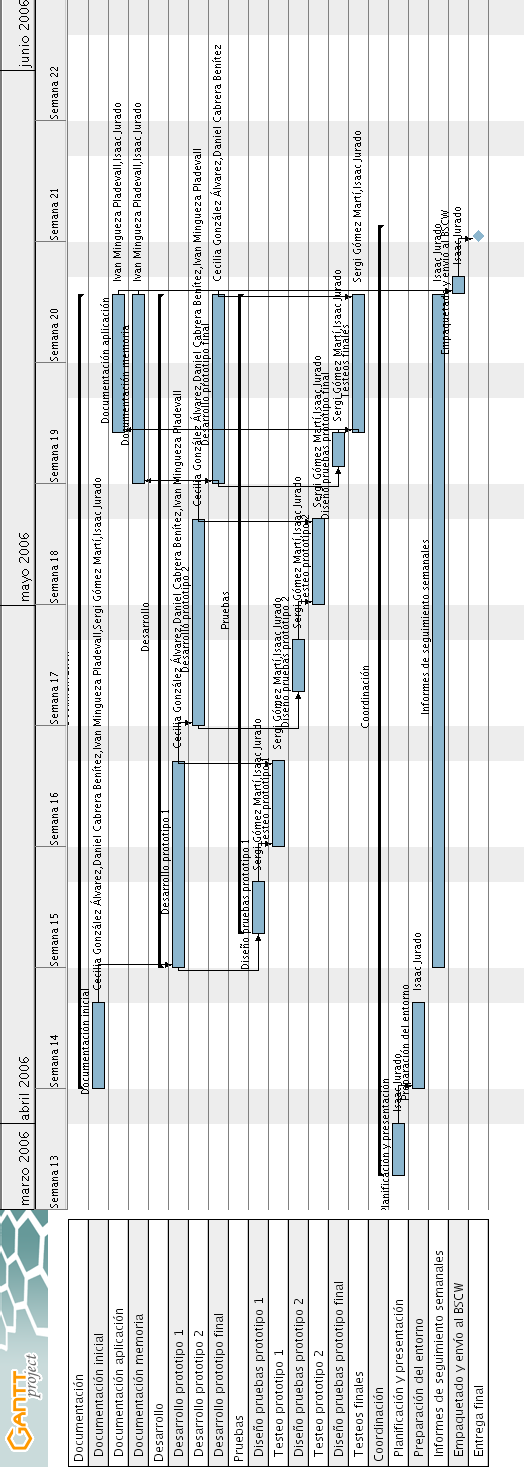
\includegraphics[height=\textheight]{gantt2}
\caption{Diagrama de Gantt para el proyecto}\label{gantt}
\end{center}
\end{figure}

\begin{figure}
\begin{center}
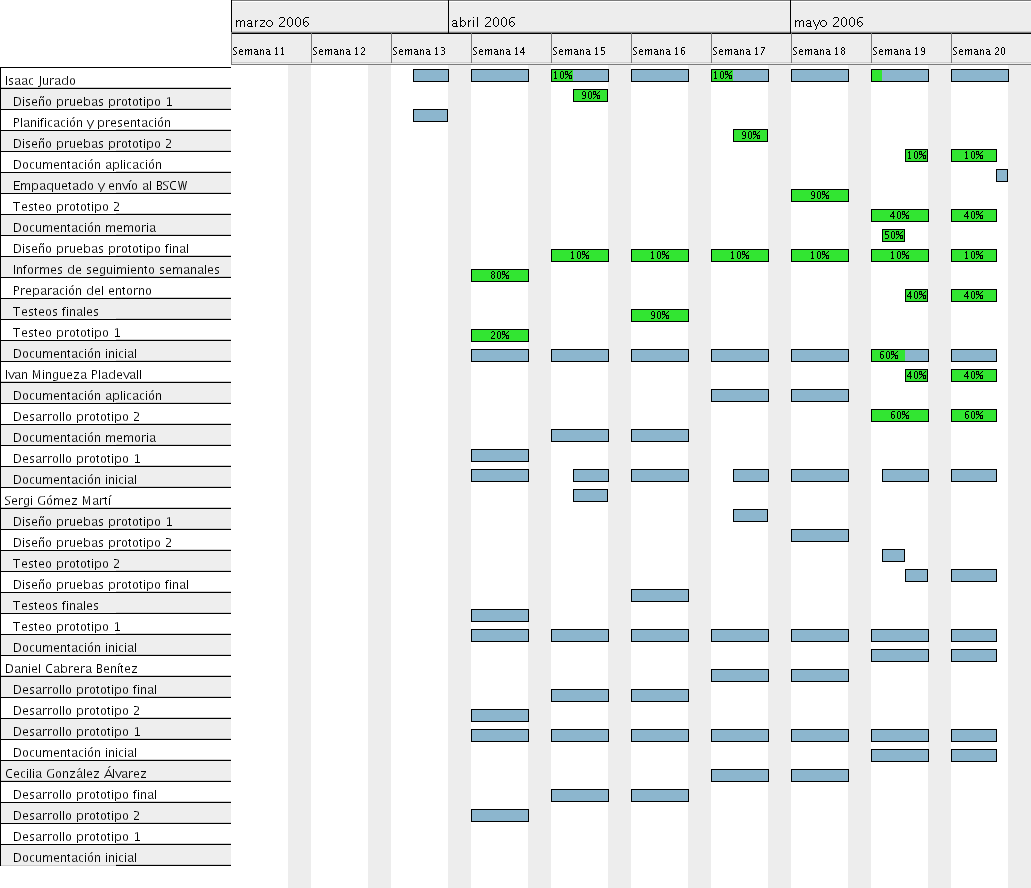
\includegraphics[width=\textwidth]{cargas}
\caption{Relación de cargas de trabajo por tarea}\label{cargas1}
\end{center}
\end{figure}


\subsection{Resultados}

El resultado final que esperamos es el programa funcionando correctamente, que
nos proporcione la posibilidad de compartir ficheros de forma sencilla e,
importante, sin necesidad de implantar mecanismos más complejos como sistemas de
ficheros remotos; lo cual requiere ciertos conocimientos avanzados de
administración y programación.


\section{Relación de la propuesta con la asignatura}

Con lo comentado en la página \pageref{tecnologias} directamente se relacionan
las tecnologías utilizadas con las vistas en la asignatura. Así que creemos
que no es necesaria ninguna justificación adicional para relacionar ambas
cosas.


\section{Paquetes de trabajo}

En los cuadros \ref{docu}, \ref{imple}, \ref{prue} y \ref{coord} se describen
con más detalle los paquetes de trabajo creados.

\begin{table}[h!]
\begin{tabular}{|r|p{0.8\textwidth}|}
\hline
\multicolumn{2}{|c|}{\emph{Paquete de Documentación}} \\
\hline
\hline

\textbf{Objetivos} &
Obtener y susminstrar información. Realizar informes y presentaciones.
Documentar la aplicación. \\
\hline
\textbf{Descripción} &
Estará pendiente a los eventos documentables importantes en el transcurso de
las otras tareas. \\
\hline
\textbf{Resultado} &
Informes, presentaciones y documentación sobre tecnologías y APIs. \\
\hline
\end{tabular}
\caption{Paquete de Documentación}\label{docu}
\end{table}

\begin{table}[h!]
\begin{tabular}{|r|p{0.8\textwidth}|}
\hline
\multicolumn{2}{|c|}{\emph{Paquete de Implementación}} \\
\hline
\hline

\textbf{Objetivos} &
Utilizar las tecnologías encontrada en la fase inicial. Desarrollar
prototipos. Corregir errores. \\
\hline
\textbf{Descripción} &
Desarrollo progresivo de prototipos a base de añadir funcionalidades y refinar
acabado. \\
\hline
\textbf{Resultado} &
La aplicación final. \\
\hline
\end{tabular}
\caption{Paquete de Implementación}\label{imple}
\end{table}

\begin{table}[h!]
\begin{tabular}{|r|p{0.8\textwidth}|}
\hline
\multicolumn{2}{|c|}{\emph{Paquete de Pruebas}} \\
\hline
\hline

\textbf{Objetivos} &
Diseñar juegos de pruebas adecuados para cada prototipo. Verificar el correcto
funcionamiento. Notificar a la implementación los errores encontrados. Volver
a aplicar las pruebas (regresión). \\
\hline
\textbf{Descripción} &
Asegurar la ausencia de errores, en la mayor medida posible, de cada prototipo
y contribuír a la corrección de los que se encuentren. \\
\hline
\textbf{Resultado} &
Juegos de pruebas y tests de regresión. Prototipos depurados. \\
\hline
\end{tabular}
\caption{Paquete de Pruebas}\label{prue}
\end{table}

\begin{table}[h!]
\begin{tabular}{|r|p{0.8\textwidth}|}
\hline
\multicolumn{2}{|c|}{\emph{Paquete de Coordinación}} \\
\hline
\hline

\textbf{Objetivos} &
Sincronizar el resto de las tareas. Asegurar el cumplimiento de los plazos.
Corregir desfases en la planificación. \\
\hline
\textbf{Descripción} &
No hace nada tangible realmente, se asegura del buen encamientamiento del
proyecto. Ayuda en la compenetración e interacción de las otras tareas. \\
\hline
\textbf{Resultado} &
Diagrama de Gantt. \\
\hline
\end{tabular}
\caption{Paquete de Coordinación}\label{coord}
\end{table}


\section{El grupo de proyecto}

\subsection{Rol de los participantes}

Como ya se comentó en clase, en general el desarrollo de todo el proyecto será
mayoritariamente anárquico. Por conveniencia vamos a particionar el grupo y
asignar recursos humanos a los distintos paquetes de trabajo. Estas
asignaciones únicamente indican quién será el mayor responsable de cada tarea
puesto que en general todos participaremos en todas las tareas.

\begin{itemize}
\item \textbf{Coordinación:} Isaac Jurado Peinado.
\item \textbf{Documentación:} Ivan Mingueza Pladevall.
\item \textbf{Desarrollo:} Daniel Cabrera Benítez y Cecilia González Álvarez. 
\item \textbf{Pruebas:} Sergi Gómez Martí. 
\end{itemize}

\subsection{Organización y gestión del proyecto}

Para gestionar el código fuente y la documentación utilizaremos mecanismos de
gestión de la configuración como el CVS\footnote{\emph{Concurrent Version
System}} que, teóricamente, los responsables de la asignatura nos deberán
proporcionar.

Las reuniones previstas coincidirán con las horas asignadas como horas de
clase. Adicionalmente nos valdremos del correo electrónico para comunicarnos
de forma extraoficial.

\end{document}

